\documentclass[12pt]{beamer}
\usecolortheme{beaver}
\usepackage[utf8]{inputenc}
\usepackage[english]{babel}
\usepackage{amssymb}
\usepackage{amsmath}
\usepackage{thumbpdf}
\usepackage{wasysym}
\usepackage{ucs}
\usepackage[utf8]{inputenc}
\usepackage{pgf,pgfarrows,pgfnodes,pgfautomata,pgfheaps,pgfshade}
\usepackage{verbatim}
\usepackage{xspace,framed,here,keystroke}
\usepackage{graphicx}
%\usepackage{minted} % Added highlighting in source code

% Enable/Disable notes - It creates a white complementary slide to help the presenter save the spech
%\setbeameroption{show notes}
%\setbeamertemplate{note page}[plain]

\setbeamertemplate {navigation symbols}{} % Remove buttons in footnote

\pdfinfo
{
  /Title       (b2llvm: B developments onto the LLVM)
  /Creator     (David Déharbe)
  /Author      (David Déharbe)
}


\title{\bllvm: B developments onto the LLVM}
\author{David Déharbe\footnote{j.w.w. R. Bonichon, T. Lecomte, V. Medeiros}}
\institute[UFRN]{Federal University of Rio Grande do Norte, Natal, Brazil}
\date{May $20^\text{\scriptsize th}$, 2014}


% Commands 

\newcommand{\trad}[2]{\ensuremath{\lVert \textsf{#1} \rVert^{\textit{#2}}}}
\newcommand{\nl}[0]{\text{\Return}}
\newcommand{\mty}[0]{\texttt{""}}
\DeclareMathOperator{\conc}{\diamond}
\DeclareMathOperator{\isdef}{\equiv}
\DeclareMathOperator{\dom}{\mbox{dom}}
\DeclareMathOperator{\name}{\mathcal{L}()}
\newcommand{\llvm}[1]{\texttt{#1}}
\newcommand{\B}[1]{\textsf{#1}}
\newcommand{\lalt}[0]{$\langle$\xspace}
\newcommand{\ralt}[0]{$\rangle$\xspace}
%\newcommand{\alt}[0]{$\mid\,$}
\newcommand{\ListOf}[1]{$\mbox{#1}^+$}
\newcommand{\nt}[1]{{\normalfont\textit{#1}}}
\newcommand{\Dict}[0]{\mathbb{D}}
\newcommand{\Text}[0]{\mathbb{T}}
\newcommand{\IF}[0]{\textbf{ if }}
\newcommand{\ELSIF}[0]{\textbf{ else if }}
\newcommand{\ELSE}[0]{\textbf{ else }}
\newcommand{\THEN}[0]{\textbf{ then }}
\newcommand{\LET}[0]{\textbf{ let }}
\newcommand{\IN}[0]{\textbf{ in }}
\newcommand{\AND}[0]{\textbf{ and }}
\newcommand{\PH}[1]{\framebox{$#1$}}
\newcommand{\sep}[0]{\otimes}
\newcommand{\intf}[0]{\ensuremath{\mathbb{I}}}
\newcommand{\Global}[0]{\ensuremath{\sf\Gamma}}
\newcommand{\local}[0]{\ensuremath{\sf\lambda}}
\newcommand{\opmap}[0]{\ensuremath{\sf\Omega}}
\newcommand{\idx}[0]{\ensuremath{\sf\Pi}}
\newcommand{\state}[0]{\ensuremath{\sf\Sigma}}
\newcommand{\tradi}[2]{\ensuremath{\langle \textsf{#1} \rangle^{\textit{#2}}}}



\begin{document}

% To enable numbered captions
\setbeamertemplate{caption}[numbered]

\frame{\titlepage}

\newcommand<>{\highlighton}[1]{%
  \alt#2{\structure{#1}}{{#1}}
}

\newcommand{\icon}[1]{\pgfimage[height=1em]{#1}}


%%%%%%%%%%%%%%%%%%%%%%%%%%%%%%%%%%%%%%%%%
%%%%%%%%%% Content starts here %%%%%%%%%%
%%%%%%%%%%%%%%%%%%%%%%%%%%%%%%%%%%%%%%%%%
\section{Introduction}

\begin{frame}

  \frametitle{Introduction}
	
\begin{minipage}{.4\textwidth}
\begin{center}
  \includegraphics[width=\textwidth]{figures/b-classic.pdf}
\end{center}
\end{minipage}
\begin{minipage}{.4\textwidth}
  \begin{itemize}
%   \item B-method: design of software \emph{components}
%     \begin{itemize}
%       \item From requirements: first-order logic, sets, integer arithmetics
%       \item To implementation: simple imperative programming language (no
%         recursion, no dynamic memory allocation).
%       \item Through: stepwise refinements and proof.
%       \end{itemize}
%   \item Atelier-B is an IDE that implements all these aspects of the B method.
%   \item There is no compiler for the B implementation language.
%   \item Instead, code in languages such as C and Ada is synthesized from
%     B implementations.
%   \item Source code synthesis is not subject to proof.
  \item \emph{Problem:\/} certify source code synthesis in Atelier-B
  \item \emph{Approach:\/} redundancy, by developing a new code generator to
    compare with.
  \end{itemize}
\end{minipage}
\end{frame}

\begin{frame}

  \frametitle{Introduction}
	
\begin{center}
  \includegraphics[width=\textwidth]{figures_minted/x_timer_i.pdf}
\vspace*{2mm}
  \includegraphics[width=\textwidth]{figures/ab-errors.pdf}
\end{center}

\begin{itemize}
\item \emph{Problem:\/} arbitrary limitations in current code synthesis
\item \emph{Approach:\/} remove limitations, keeping in mind application
  context.
\end{itemize}
\end{frame}

\begin{frame}

  \frametitle{The \bllvm project}
	
\begin{minipage}{.34\textwidth}
  \includegraphics[width=\textwidth]{figures/b-llvm.pdf}
\end{minipage}
\begin{minipage}{.56\textwidth}
  \includegraphics[width=\textwidth]{figures/b-certify.pdf}
\end{minipage}

  \begin{itemize}
  \item Code synthesis for B targeting LLVM.
  \item Working prototype.
  \end{itemize}

\end{frame}

\section{LLVM}

\begin{frame}
\frametitle{LLVM}

\begin{quote}
``The LLVM Project is a collection of modular and reusable compiler and toolchain technologies.'' (\url{http://www.llvm.org})
\end{quote}

\begin{itemize}
\item Used in many commercial and open-source projects
\begin{itemize}
\item Adobe, Apple, Cray, Intel, NVIDIA 
\end{itemize}
\item Used in academic research
\begin{itemize}
\item \emph{Formalizing the LLVM Intermediate Representation for Verified Program Transformations}. J. Zhao, S. Nagarakatte, M. Martin, S. Zdancewic. POPL 2012.
\end{itemize}
\item backbone of LLVM: an \emph{assembly language}
\begin{itemize}
\item an intermediate representation (IR)
\item generated by compiler front-ends (parsing, type analysis) 
\item consumed, transformed by back-ends (optimization, target code
  generation).
\end{itemize}
\end{itemize}
	
\end{frame}

\begin{frame}
\frametitle{LLVM-IR}

\begin{itemize}
\item Example
\begin{center}
\begin{tabular}[t]{cc}
  C & LLVM \\
  \includegraphics{figures_minted/x_inc_c.pdf}&
  \includegraphics{figures_minted/x_inc_llvm.pdf}
\end{tabular}
\end{center}
\item Single-static assignment
\item Strongly typed
\item Modular
\end{itemize}

\end{frame}

\begin{frame}{LLVM module items}

\begin{itemize}
\item type declaration

\noindent\includegraphics{figures_minted/x_typedecl.pdf}
\item Type definitions

\noindent\includegraphics{figures_minted/x_typedef.pdf}
\item constant declaration

\noindent\includegraphics{figures_minted/x_constdecl.pdf}
\item constant definition

\noindent\includegraphics{figures_minted/x_constdef.pdf}
\item function declaration

\noindent\includegraphics{figures_minted/x_fundecl.pdf}

\item function definition...
\end{itemize}

\end{frame}

\begin{frame}{LLVM function definitions}

\noindent\includegraphics[width=\textwidth]{figures_minted/x_fundef1.pdf}

\end{frame}

\begin{frame}

  \frametitle{Some remarks on the B method}
	
  \begin{itemize}
  \item Construction of software \emph{modules\/}.
  \item A module may be
    \begin{itemize}
    \item a \emph{developed} module: implementation derived in B.
    \item a \emph{base} module: implementation derived outside of B.
    \end{itemize}
  \item A developed module has a B specification (machine) and a B
    implementation.
  \item A base module has a B specification (machine).
  \item A B module may \emph{import} other modules.
  \item A root B module may (transitively) contain several instances of other
    B modules.
  \end{itemize}

\end{frame}

\begin{frame}

  \frametitle{Some general requirements}
	
  \begin{itemize}
  \item No dynamic memory allocation
    \begin{itemize}
    \item This is a requirement in some applications (often
      safety-critical systems).
    \item No need for a third-party library.
    \end{itemize}
  \item Separate code generation
    \begin{itemize}
    \item This is a requirement for large projects.
    \item Internal changes in a B module shall only require generating code
      for that module.
    \item Changes in the interface of a B module requires generating code
      for that module and those other modules that use it.
    \end{itemize}
  \end{itemize}

\end{frame}

\begin{frame}{Code generation}

  \begin{itemize}
  \item Specified as a set of code generation rules\footnote{You will be spared a detailed presentation of the rules.}

    \includegraphics[width=.75\textwidth]{rule.pdf}
  \item Validated via 
    \begin{itemize}
    \item trial encoding
    \item rapid prototyping
      \begin{itemize}
      \item read XML files produced by a third-party tool
      \item Python
      \end{itemize}
    \end{itemize}
  \end{itemize}
  

\end{frame}

\begin{frame}{B constructs}

  \begin{itemize}
    \item Constants, variables
    \item Module instantiation (imports) \only<2>{\alert{$\leftarrow$ More on this}}
    \item Imperative constructs: conditionals, loop, local variables, assignments, operation calls.
    \item Arithmetic and relational expressions, conditionals
    \item Integers, Booleans, Enumerations.
    \item \textcolor{red}{-} lambda expressions, arrays, records,
    \item \textcolor{red}{- -} machine parameters.
  \end{itemize}
\end{frame}


\begin{frame}

  \frametitle{B projects and code generation}
	
  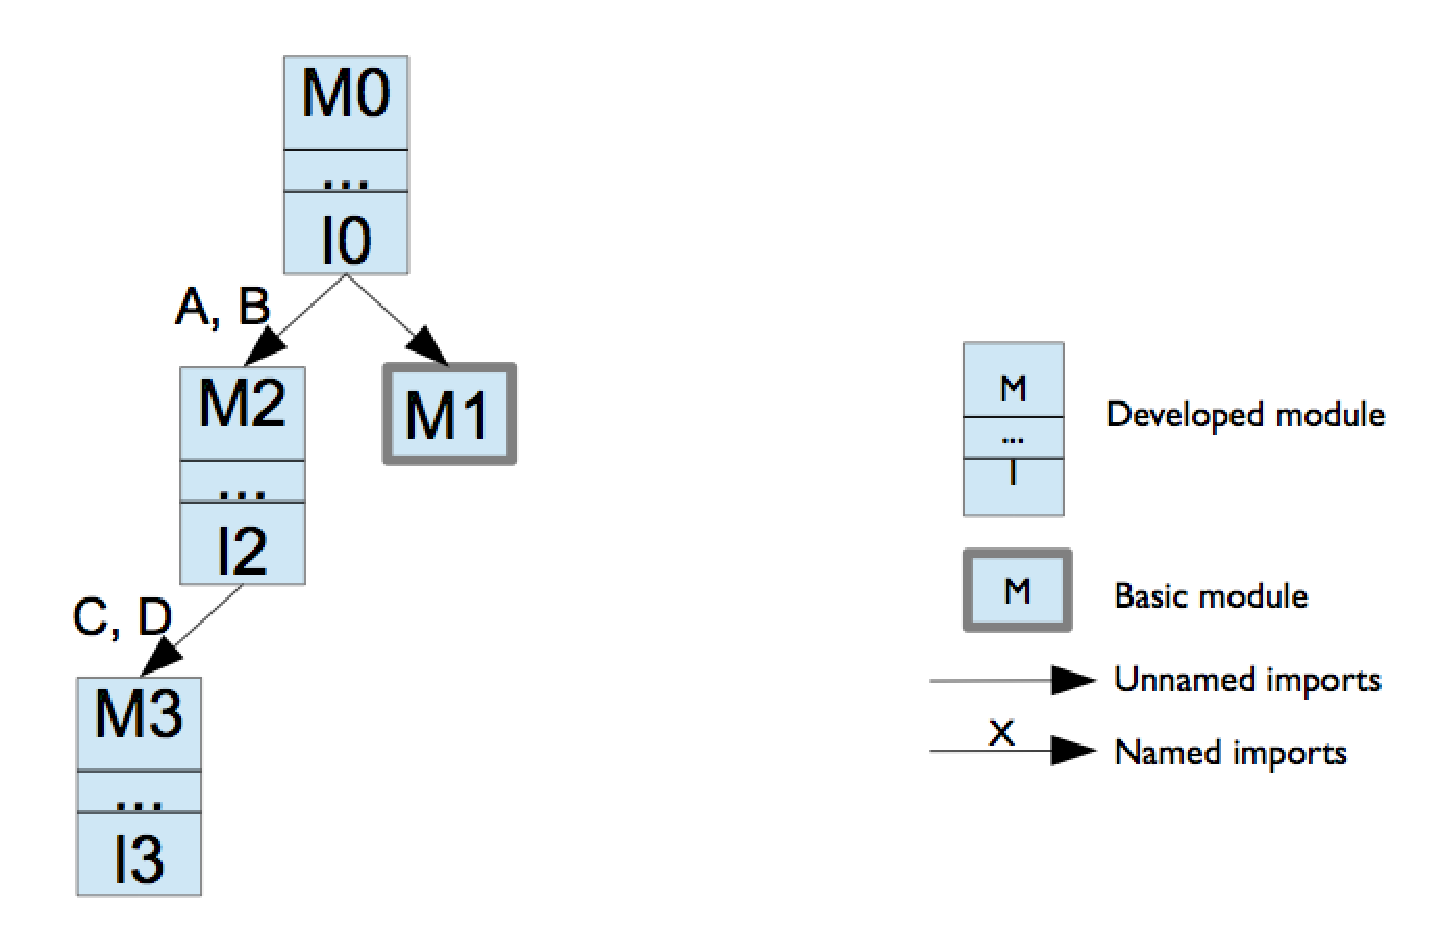
\includegraphics[height=.4\textheight]{B-project.pdf}

  To build the project LLVM code:
  \begin{description}
  \item[b2llvm] \alert{component} mode:
    \begin{itemize}
      \item \B{M0} \B{M2} \B{M3} $\Longrightarrow$ \llvm{m0.ll} \llvm{m2.ll} \llvm{m3.ll} 
    \end{itemize}
  \item[b2llvm] \alert{project} mode:
    \begin{itemize}
      \item \B{M0} $\Longrightarrow$ \llvm{init-m0.ll}
    \end{itemize}
  \item[LLVM] optimize, generate assembly, link
    \begin{itemize}
      \item \llvm{init-m0.ll} \llvm{m0.ll} \llvm{m2.ll} \llvm{m3.ll} \textcolor{red}{\llvm{m1.o}} $\Longrightarrow$ \llvm{a.out}
      \end{itemize}
  \end{description}
\end{frame}


\begin{frame}

  \frametitle{Bricks of LLVM code}
	
{
\newcommand{\myind}{\hspace*{2em}}
\small
\begin{minipage}{.9\textwidth}
\noindent\textbf{type def:}
A structure type (one item per state variable and import): 
\textcolor{blue}{\llvm{\%M\$state\$ = type \{ \ListOf{\nt{type}} \}}} \\
\\
\noindent\textbf{type decl:}
\textcolor{blue}{\llvm{\%M\$state\$ = type opaque}} \\
\\
\noindent\textbf{type ref:}
A pointer type: 
\textcolor{blue}{\llvm{\%M\$ref\$ = type \%M\$state\$*}} \\
\\
\noindent\textbf{function decl:} 
An initialization function:\\
\textcolor{blue}{\llvm{declare void @M\$init\$(\%M\$ref\$, \ListOf{\nt{type}})}} \only<2>{\alert{$\leftarrow$ address of module instance}}\\
One function for each operation in the module: \\
\textcolor{blue}{\llvm{declare void @M\$op(\%M\$ref\$, \ListOf{\nt{type}})}}\\
\\
\noindent\textbf{function def:}
(for developed modules): \\
\textcolor{blue}{\llvm{define void @M\$op(\%M\$ref\$ \%self\$, \ListOf{\nt{param}}) \{}} \\
\myind \textcolor{blue}{\llvm{\ListOf{\nt{block}}}} \\
\myind \textcolor{blue}{\llvm{exit: ret void}} \\
\textcolor{blue}{\llvm{\}}}
\end{minipage}
}

\end{frame}

\begin{frame}

  \frametitle{Example 1}

  \begin{center}
    \includegraphics{figures_minted/x_count_i.pdf}
  \end{center}

  \begin{itemize}
    \item type definition

{\small \textcolor{blue}{\llvm{\%counter\$state\$ = type \{ i32, i1 \}}}}
    \item reference type

{\small \textcolor{blue}{\llvm{\%counter\$ref\$ = type \%counter\$state\$*}}}
    \item function declarations:

{\small
      \textcolor{blue}{\llvm{declare void @counter\$init\$(\%counter\$ref\$)}}

      \textcolor{blue}{\llvm{declare void @counter\$inc(\%counter\$ref\$)}}

      \textcolor{blue}{\llvm{declare void @counter\$get(\%counter\$ref\$, i32*)}}
}
    \end{itemize}
\end{frame}

\begin{frame}

  \frametitle{Example 1 (a function definition)}

  \includegraphics{figures_minted/count_i-inc.pdf}
  
  \vspace*{-10mm}
  \includegraphics{figures_minted/count_i_llvm_inc.pdf}

\end{frame}

\begin{frame}

  \frametitle{Example 1 (another function definition)}

  \includegraphics{figures_minted/count_i-get.pdf}
  
  \vspace*{-10mm}
  \includegraphics{figures_minted/count_i_llvm-get.pdf}

\end{frame}

\begin{frame}

  \frametitle{Example 2}

  \begin{center}
    \includegraphics[height=.5\textheight]{figures_minted/x_wd_i.pdf}
  \end{center}

  \begin{itemize}
    \item type definition

{\small \textcolor{blue}{\llvm{\%wd\$state\$ = type \{ \%count\$ref\$ \}}}}
    \item function declarations:

    \includegraphics{figures_minted/x_wd_i_llvm-fun-decl.pdf}

    \end{itemize}
\end{frame}

\begin{frame}

  \frametitle{Example 2 (definition of function for initialization)}

  \includegraphics{figures_minted/x_wd_i_llvm-init-def.pdf}

\end{frame}

\begin{frame}

  \frametitle{Putting it all together: component mode}

  \begin{itemize}
  \item type definition
    \begin{itemize}
    \item need type references of imported modules
    \end{itemize}
  \item function definitions
    \begin{itemize}
    \item need type references of transitively imported
      modules (initialization)
    \item need function declarations of imported modules
      (operation calls, initialization)
    \end{itemize}
  \end{itemize}

\end{frame}

\begin{frame}

  \frametitle{Putting it all together: project mode}

  \begin{itemize}
    \item to create instances of all the instances of all the
      modules:
      \begin{itemize}
        \item type definition of module
        \item type reference of module
        \item type definitions of transitively imported modules
        \item type references of transitively imported modules
      \end{itemize}
      For each instance \B{Q} of a module \B{M}

      {\small 
        \textcolor{blue}{\llvm{@\$Q[path] = common global @\$Q\$state\$ zeroinitializer}}}

    \item to initialize the system:
      \begin{itemize}
      \item function declaration (initialization)
        of the module
      \end{itemize}

      {\small 
        \textcolor{blue}{\llvm{define void @\$init\$(void) \{}}

        \textcolor{blue}{\llvm{\hspace*{.5cm} call void @M\$init\$(\$M, ...)}}

        \textcolor{blue}{\llvm{\hspace*{.5cm} ret void}}

        \textcolor{blue}{\llvm{\}}}
        }

  \end{itemize}

\end{frame}

\begin{frame}{Putting it all together: project for example 2}

  \includegraphics{figures_minted/x_wd_llvm_main.pdf}

\end{frame}

% \begin{frame}{extra}
%   For each B module \B{M}, generate code for
%   \begin{description}
%   \item[typedef] An LLVM record type \llvm{@M\$state\$} to represent the state
%     of the module, with
%     \begin{itemize}
%     \item one record field for each state variable;
%     \item one record field for each imported module.
%     \end{itemize}
%   \item An LLVM pointer type \llvm{@M\$ref\$} to represent pointers to 
%     \llvm{@M\$state\$}.
%   \item A LLVM function \llvm{@M\$init\$} to initialize module instances,
%     \begin{itemize}
%     \item parameter: the (representation) of the instance to be initialized
%     \item extra parameters: the (representation) of the component instances.
%     \end{itemize}
%   \item one LLVM function \llvm{@M\$op\$} for each operation \B{op} in \B{M}.
%     \begin{itemize}
%     \item parameter: the (representation) of the called instance.
%     \item extra parameters: the inputs and the outputs of the operation.
%     \end{itemize}
%   \end{itemize}

% \end{frame}

\begin{frame}{Verification, validation}

\begin{itemize}
  \item Formal verification:
    \begin{itemize}
    \item Formalize LLVM-IR (available)
    \item Formalize B (partly available)
    \item Formalize and verify code generation rules (to be done)
    \end{itemize}
  \item Assertions in generated code.
    \begin{itemize}
    \item Implement assert in LLVM.
    \item Define code generation rules for full conditions (not only
      implementable conditions).
    \end{itemize}
  \item Test generated code (ongoing work)
  \item Generate debugging aids (some done)
  \item Traceability (done)
\end{itemize}

\end{frame}

\begin{frame}{Traceability: an example}

\includegraphics{figures_minted/x_with_trace.pdf}

\end{frame}

\section{Conclusion}

\begin{frame}{Conclusion}

\begin{itemize}
\item \bllvm is open-source (\url{http://www.b2llvm.org/b2llvm}).
\item \bllvm is compatible with Atelier-B 4.2 (availability: June 2014).
\item Available validation strategies: 
\begin{itemize}
\item output code may be annotated.
\item debugging code may be generated.
\end{itemize}
\end{itemize}
\end{frame}

\begin{frame}{Ongoing work}
\begin{itemize}
\item lambda terms;
\item support to type constructors: arrays, records;
\item integration with test-generation tool.
\end{itemize}

\end{frame}

\begin{frame}

\begin{center}
\huge ?
\end{center}

\end{frame}

\begin{frame}[fragile]
  \frametitle{Syntax of the target LLVM-IR: module elements}

  \begin{center}
    \begin{tabular}{rcl}
      \nt{module} & ::= & \ListOf{\nt{item}} \\
      \nt{item} & ::= &  \nt{type\_def} \ALT \nt{const\_decl} \ALT \nt{const\_def} \ALT \nt{var\_def}\\
      & & \ALT \nt{function\_decl} \ALT \nt{function\_def} \\
      \nt{type\_def} & ::= & \nt{name} \llvm{=} \llvm{type} \nt{type} \\
      \nt{type} & ::= & \llvm{void} \ALT \nt{itype} \ALT \llvm{\{} \ListOf{\nt{type}} \llvm{\}} \ALT \nt{type}\llvm{*} \ALT \llvm{opaque} \\
      \nt{const\_decl} & ::= & \nt{name} \llvm{=} \llvm{external} \llvm{constant} \nt{type} \\
      \nt{const\_def} & ::= & \nt{name} \llvm{=} \llvm{constant} \nt{type} \nt{iliteral} \\
      \nt{var\_def} & ::= & \nt{name} \llvm{=} \llvm{common} \llvm{global} \nt{type} \llvm{zeroinitializer} \\
      \nt{function\_decl} & ::= & \llvm{declare} \nt{type} \nt{name} \llvm{(} \ListOf{\nt{type}} \llvm{)}\\
      \nt{function\_def} & ::= & \llvm{define} \nt{type} \nt{name} \llvm{(} \ListOf{\nt{param}} \llvm{)} \llvm{\{} \ListOf{\nt{block}} \llvm{\}} \\
      \nt{param} & ::= & \nt{type} \nt{name} \\
      \nt{block} & ::= & \nt{lbl} \llvm{:} \ListOf{\nt{inst}}
    \end{tabular}
  \end{center}

\end{frame}

\begin{frame}[fragile]
  \frametitle{Syntax of the target LLVM-IR: instructions}

  \begin{center}
    \begin{tabular}{rcl}
      \nt{inst} & ::=  & \nt{name} \llvm{=} \llvm{alloca} \nt{type} \\
      & \ALT & \nt{name} \llvm{=} \nt{arith} \nt{itype} \nt{exp} \llvm{,} \nt{exp} \\
      & \ALT & \nt{name} \llvm{=} \llvm{icmp} \nt{rel} \llvm{i1} \nt{exp} \llvm{,} \nt{exp}\\
      & \ALT & \nt{name} \llvm{=} \llvm{call} \nt{type} \llvm{(} \ListOf{\nt{arg}} \llvm{)} \\
      & \ALT & \nt{name} \llvm{=} \llvm{getelementptr} \nt{type} \llvm{*} \nt{exp}\llvm{,} \nt{index}\llvm{,} \nt{index}  \\
      & \ALT & \nt{name} \llvm{=} \llvm{load} \nt{type} \nt{exp} \\
      & \ALT & \llvm{store} \nt{type} \nt{exp}, \nt{type} \llvm{*} \nt{exp} \\
      & \ALT & \llvm{br} \llvm{i1} \nt{exp} \llvm{,} \llvm{label} \nt{lbl} \llvm{,} \llvm{label} \nt{lbl} \\
      & \ALT & \llvm{br} \llvm{label} \nt{lbl} \\
      & \ALT & \llvm{switch} \nt{type} \nt{exp} \llvm{,} \llvm{branch} \nt{lbl} \llvm{[} \ListOf{\nt{branch}} \llvm{]} \\
      & \ALT & \llvm{ret} \nt{type} \nt{exp}\\
      & \ALT & \llvm{ret} \llvm{void} \\
    \end{tabular}
  \end{center}

\end{frame}

\begin{frame}[fragile]
  \frametitle{Syntax of the target LLVM-IR: expressions, misc.}

  \begin{center}
    \begin{tabular}{rcl}
      \nt{arith} & ::= & \llvm{add} \ALT \llvm{sub} \ALT \llvm{mul} \ALT \llvm{sdiv} \ALT \llvm{srem} \\
      \nt{rel} & ::= & \llvm{eq} \ALT \llvm{ne} \ALT \llvm{sgt} \ALT \llvm{sge} \ALT \llvm{slt} \ALT \llvm{sle} \\
      \nt{exp} & ::= & \nt{name} \ALT \nt{iliteral} \ALT \\
& & \llvm{getelementptr} \llvm{(} \nt{type} \nt{exp} \llvm{,} \nt{index} \llvm{,} \nt{index} \llvm{)} \\
      \nt{index} & ::= & \nt{itype} \nt{iliteral} \\
      \nt{branch} & ::= & \nt{iliteral} \nt{iliteral} \nt{lbl} \\
      \nt{arg} & ::= & \nt{type} \nt{exp}
    \end{tabular}
  \end{center}

Main missing construct: arrays.

\end{frame}

\begin{frame}{Example 1 (standalone module)}

  \begin{center}
    \includegraphics{figures_minted/x_count_i.pdf}
  \end{center}
\end{frame}

\begin{frame}{Example 2 (composed module)}

  \begin{center}
    \includegraphics{figures_minted/x_wd_i.pdf}
  \end{center}
\end{frame}

\begin{frame}

  \frametitle{B projects and code generation}
	
  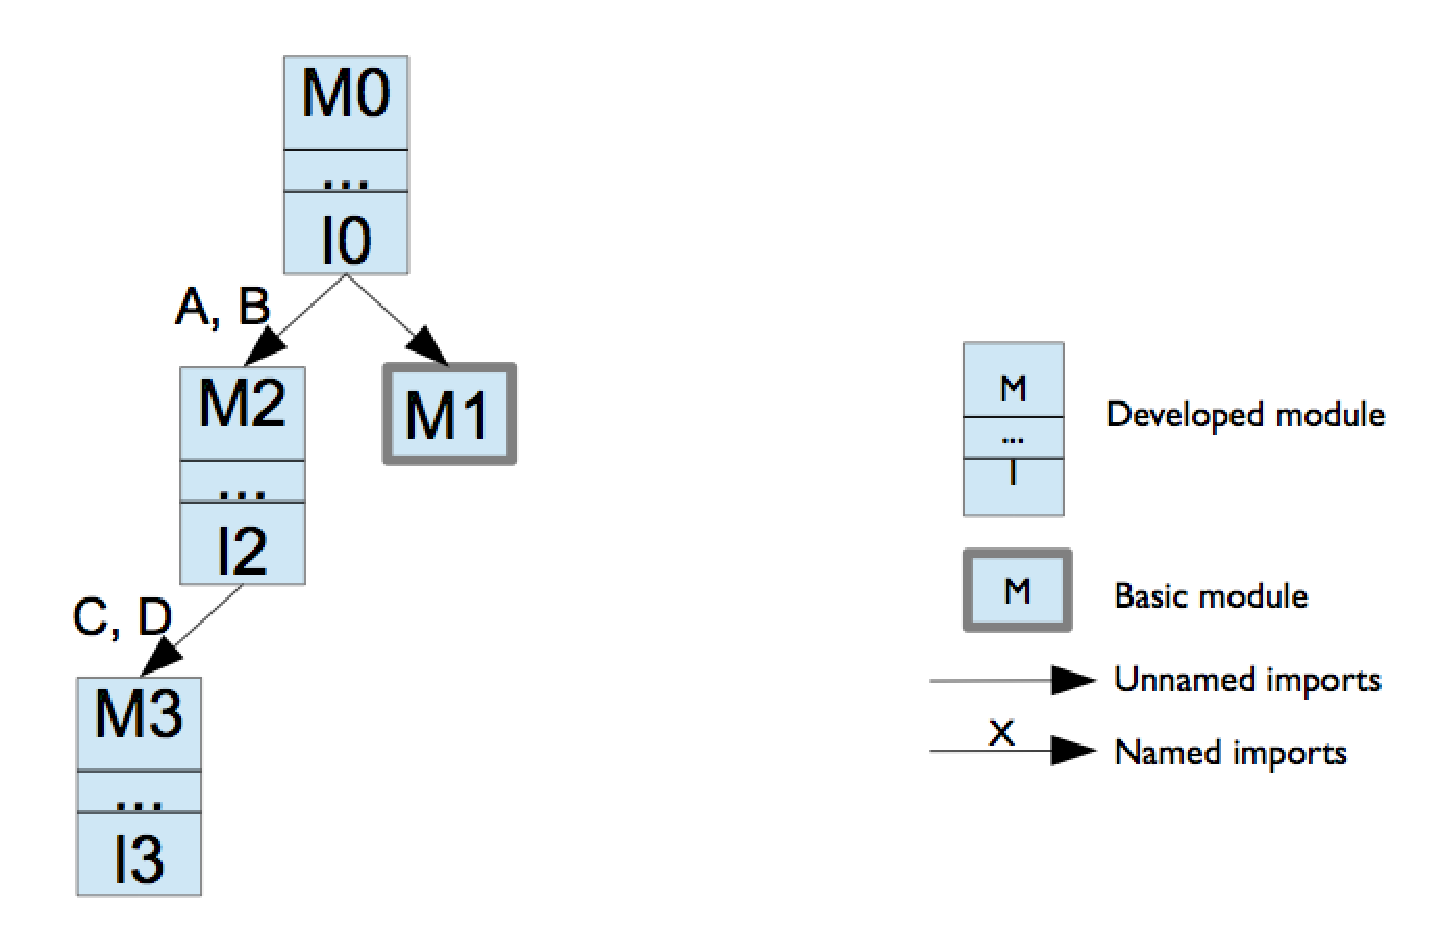
\includegraphics[height=.4\textheight]{B-project.pdf}
  \begin{enumerate}
  \item modules access other modules (base or developed) through their interface
    $\Longrightarrow$ need to generate LLVM for module \emph{interface}.
  \item Memory for each instance of each \B{Mi} must be allocated statically
    $\Longrightarrow$ global variables.
  \item Instances should be created only when the full project is compiled
    $\Longrightarrow$ two code generation modes: \emph{component} and 
    \emph{project}.
  \end{enumerate}
\end{frame}

\end{document}

